\documentclass[slovene]{book}
\usepackage{amsmath} 
\usepackage{amssymb} 
\usepackage{makeidx} 
\usepackage{graphicx} 
\usepackage{epstopdf}
\graphicspath{{img/}}

\usepackage{url}
\usepackage{babel}
\usepackage[T1]{fontenc}
\usepackage[cp1250]{inputenc}

\usepackage{color}
\usepackage[normalem]{ulem}
% define red
\newcommand{\red}[1]{\textcolor{red}{#1}}

%\includeonly{chaptr2} %If you just want to process chaptr2.tex

%%%
% new commands
%%%

\newcommand{\eng}[1]{(angl.~\emph{#1})}

%%%
% definicija
%%%

\newtheorem{definicija}{Definicija}

%%%
% Zgled
%%%

\newtheorem{zgled}{Zgled}

%%%
% document
%%%

\begin{document}

\author{Uredil prof. dr. Miha Mraz}
\title{Analiza zmogljivosti obla�nih in stre�ni�kih storitev}
\date{Maj 2015}
\maketitle

\frontmatter
\tableofcontents

\chapter{Predgovor}


Pri�ujo�i uvod bom napisal naknadno.


prof.dr. Miha Mraz, Ljubljana maj 2015



\mainmatter

\chapter[Zmogljivostna analiza ogla�evalskega sistema (A. Lampe,  D. �tepec, A. Medved)]{Zmogljivostna analiza ogla�evalskega sistema}
\huge Ajda Lampe, Dejan �tepec, An�e Medved\\
\normalsize
\bigskip

\section{Slike}
Slike pripravite v EPS formatu. Na sliki  \ref{fig:poglavje2_ac} je za zgled navedena ena slika Petrijevih mre�.

\begin{figure}[htbf]
\begin{center}
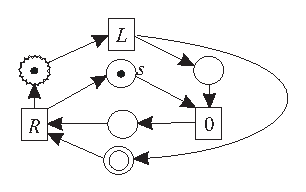
\includegraphics{poglavje2_ac}
\end{center}
\caption{Model popravljive entitete, ki za servisiranje zahteva prisotnost resursa $s$.}
\label{fig:poglavje2_ac}
\end{figure} 

\section{Tekst}
Poleg ukaza section lahko uporabljate tudi ukaze subsection in subsubsection (le v izjemnih primerih). Nadaljnja vejanja so neza�eljena. Pa �e ena ena�ba, ki jo najdemo v izrazu (\ref{sklic})
\begin{equation}
A\text{ / }B\text{ / }m\text{ / }k\text{ / }P\text{,}\label{sklic}%
\end{equation}
seveda pa ne bo �lo tudi brez na�tevanja:

\begin{itemize}
\item \textit{A}: verjetnostna porazdelitev medprihodnih \v{c}asov vstopajo\v{c}ih zahtev,
\item \textit{B}: verjetnostna porazdelitev stre\v{z}nih \v{c}asov zahtev.
\end{itemize}

\section{Citiranje}
V prilo�eni datoteki mro.bib imate vzorce, kako kak�ne reference (vire) zabele�iti v taisto datoteko. V viru \cite{sch1} najdemo kar nekaj zanimivosti o Petrijevih mre�ah.

 % 1.Poglavje

\backmatter
%\include{glossary}
%\include{notat}
\bibliographystyle{ieeetr} %The style you want to use for references.
\bibliography{mro} %The files containing all the articles and books you ever referenced.
\printindex %Make an index AUTOMATICALLY

\end{document} 
